\chapter{Базы данных}
\label{ch:databases}

\newthought{App Inventor поддерживает работу} с онлайн базами данных. 
И база TinyWebDB, и база данных 
Google Fusion Tables (<<ДинамиТ>>% 
\footnote[][-1.0cm]{
        Google Fusion Tables в русском интерфейсе среды App Inventor называется 
        ужасно длинно: <<УправлениеДинамическимиТаблицами>>, 
        будем эту базу данных называть просто и взрывно -- <<ДинамиТ>>. 
}) имеют свои ограничения.
База данных TinyWebDB более простая в использовании, 
но любой, кто получит доступ к базе, может изменить её содержимое. 
Несмотря на название, база ДинамиТа более безопасна, но сложнее в освоении. 

Великолепная четвёрка в 2011 году написала о работе с базами данных 
TinyDB и TinyWebDB\cite{Giesemann2020}. 
\marginnote[-0cm]{
    В книге 2011 года этим базам посвящена целая глава, доступная онлайн: 
    \href{http://www.appinventor.org/bookChapters/chapter22.pdf}{Working with Databases}.
}
В книге, написанной Камриани и Роем\cite{KamrianiAndRoy2016}, 
рассказывается о работе с базой данных ДинамиТ. 

Чтобы добраться до элементов баз данных в среде App Inventor, 
нажмите кнопку <<Дизайнер>>. 
Затем в меню <<Палитры>> разверните панель <<Хранилище>> и увидите 
список доступных способов долговременного хранения данных (рис.~\ref{fig:storage_and_db_types}): 
\begin{itemize}
    \item Файл,
    \item УправлениеДинамическимиТаблицами,
    \item TinyDB,
    \item TinyWebDB.
\end{itemize}

\begin{marginfigure}[0.3cm]
{%
\setlength{\fboxsep}{0pt}%
\setlength{\fboxrule}{1pt}%
\fcolorbox{gray}{gray}{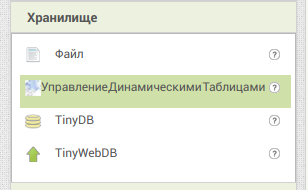
\includegraphics{./lessons/db_google_fusion/01_storage_and_db_types.png}}%
}%
%
\includegraphics{./commons/Flag_of_Republika_Srpska.png}
    \caption{В <<Дизайнере>> в меню <<Палитра>> развёрнута вкладка <<Хранилище>> 
    со списком доступных способов хранения данных: файл и три базы данных}
\label{fig:storage_and_db_types}
\end{marginfigure}

Справа от названия типа хранилища есть значок вопроса (рис.~\ref{fig:storage_and_db_types}). 
Если нажать на значок, то всплыёт окно с подсказкой и рассказом, 
что это за база и как с ней работать.

Вопросы (todo answers and goto links): 
\begin{itemize}
    \item Назовите сайты и программы, которым необходима для работы база данных.
    \item Почему переменная называется <<переменной>> или по-английски ``variable''? 
        Данные в базе являются переменными или константами?
    \item Кто дольше живёт ‒ переменная или константа? (упомянуть рассказ Лема о роботе-дубликате, 
    который симулировал работу, чтобы его не выключили)
    \item Зачем хранить данные в базе данных, если уже есть переменные?
\end{itemize}
